
前面的一节中,了解了如何在Clang中表示源位置,而源位置是预处理器的重要组成部分。本节中,将首先解释Clang的预处理器和词法分析器的原理,以及工作流程。然后,了解这个流程中的一些重要组件,并简要解释它们的用法。

\subsubsubsection{6.3.1\hspace{0.2cm}Clang中预处理器和词法分析器的作用}

Clang的预处理器和词法分析器执行的角色和主要操作,分别由\texttt{Preprocessor}和\texttt{Lexer}类表示,如下图所示:

\hspace*{\fill} \\ %插入空行
\begin{center}
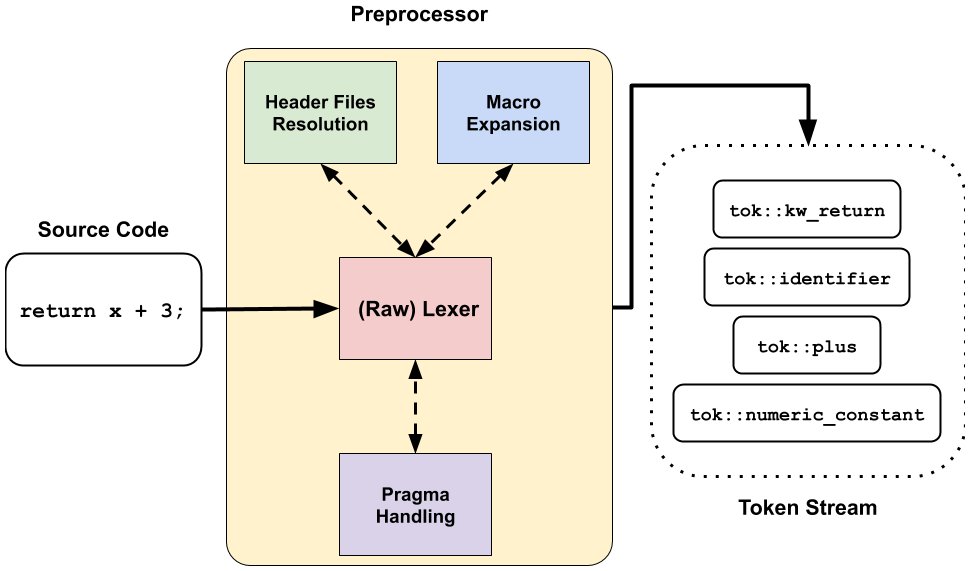
\includegraphics[width=0.9\textwidth]{content/2/chapter6/images/1.png}\\
图6.1 - Clang预处理器和词法分析器的角色
\end{center}

相信大多数读者都熟悉词法分析器上下文中的\textbf{令牌}概念——源自原始源代码的子字符串,并充当语义推理的最小构建块。在一些传统的编译器中,分析器负责将输入的源代码切成一个令牌序列或\textbf{令牌流}(如上图所示),这个令牌流稍后将被提供给解析器以构造语义结构。

实现方面,Clang采取了与传统编译器(或教科书上的编译器)不同的路径:\texttt{Preprocessor}使用的\texttt{Lexer}仍然是将源代码划分成令牌的主要执行者。然而,每当遇到预处理器指令(即任何以\texttt{\#}开头的指令)或符号时,\texttt{Lexer}都不会干涉,并将该任务转发给宏展开、头文件解析器或由预处理器组织的编译处理器。如果需要,这些辅助组件会将额外的令牌注入到主令牌流中,这些令牌流最终会返回给使用\texttt{Preprocessor}的用户。

换句话说,令牌流的大多数“消费者”并不直接与\texttt{Lexer}交互,而是与\texttt{Preprocessor}实例交互。因为\texttt{Lexer}本身只生成一个没有经过预处理的令牌流,这使得\texttt{Lexer}类被称为原始\texttt{Lexer}(如前面的图所示)。为了更具体地了解如何使用因为\texttt{Lexer}本身只生成一个没有经过预处理的令牌流\texttt{Preprocessor}来检索令牌(流),我们提供了以下简单的代码片段,其会显示从当前处理的源代码中获取下一个令牌的方法:

\begin{lstlisting}[style=styleCXX]
Token GetNextToken(Preprocessor &PP) {
	Token Tok;
	PP.Lex(Tok);
	return Tok;
}
\end{lstlisting}

你可能已经猜到的,\texttt{Token}是Clang中的单个令牌类,我们将在下一段中对其进行介绍。

\subsubsubsection{6.3.2\hspace{0.2cm}Token类}

\texttt{Token}类是单个令牌的表示,这些令牌可以来自源代码,也可以来自用于特殊目的的虚拟令牌。其也应用于预处理/词法分析框架,就像我们前面介绍的\texttt{SourceLocation}一样。因此,需要设计成内存简洁和可复制的类型。

对于\texttt{Token}类,在这里要强调两件事:

\begin{enumerate}
\item \textbf{令牌类型}描述了这个令牌是什么。
\item \textbf{标识符}表示语言关键字和任意前端标记(例如函数名)。Clang的预处理器使用了\texttt{IdentifierInfo}类来携带额外的标识符信息,将在本节的后面介绍这些信息。
\end{enumerate}

\hspace*{\fill} \\ %插入空行
\noindent
\textbf{令牌类型}

令牌类型描述了这个\texttt{Token}是什么。Clang的\texttt{Token}不仅用于表示具体的、物理语言结构,如:关键字和符号,还用于表示由解析器插入的虚拟概念,以便使用单个\texttt{Token}编码具有尽可能多的信息。要查看令牌流的类型,可以使用以下命令行选项:

\begin{tcblisting}{commandshell={}}
$ clang -fsyntax-only -Xclang -dump-tokens foo.cc
\end{tcblisting}

\texttt{foo.cc}文件内容如下所示:

\begin{lstlisting}[style=styleCXX]
namespace foo {
	class MyClass {};
}
foo::MyClass Obj;
\end{lstlisting}

输出信息如下:

\begin{tcblisting}{commandshell={}}
namespace 'namespace' [StartOfLine] Loc=<foo.cc:1:1>
identifier 'foo' [LeadingSpace] Loc=<foo.cc:1:11>
l_brace '{' [LeadingSpace] Loc=<foo.cc:1:15>
class 'class' [StartOfLine] [LeadingSpace] Loc=<foo.
cc:2:3>
identifier 'MyClass' [LeadingSpace] Loc=<foo.cc:2:9>
l_brace '{' [LeadingSpace] Loc=<foo.cc:2:17>
	r_brace '}' Loc=<foo.cc:2:18>
semi ';' Loc=<foo.cc:2:19>
r_brace '}' [StartOfLine] Loc=<foo.cc:3:1>
identifier 'foo' [StartOfLine] Loc=<foo.cc:5:1>
coloncolon '::' Loc=<foo.cc:5:4>
identifier 'MyClass' Loc=<foo.cc:5:6>
identifier 'Obj' [LeadingSpace] Loc=<foo.cc:5:14>
semi ';' Loc=<foo.cc:5:17>
eof '' Loc=<foo.cc:5:18>
\end{tcblisting}

起始部分是每个令牌的令牌类型。完整的令牌类型列表可以在\texttt{clang/include/clang/Basic/\\Tokenkings.def}中找到。这个文件是一个参考,可以了解语言结构(例如,\texttt{return}关键字)与其对应的令牌类型(\texttt{kw\_return})的映射。

虽然无法可视化虚拟标记(或者注释标记,因为它们在Clang的代码库中被调用),但我们仍将使用与前面相同的示例来解释这些标记。在C++中,\texttt{::}(前面指令中的\textit{冒号}标记类型)有几种不同的用法,例如:可以用于命名空间解析(在C++中更正式的说法是作用域解析),如前面的代码片段所示,也可以(可选地)与\texttt{new}和\texttt{delete}操作符一起使用,如下面的代码所示:

\begin{lstlisting}[style=styleCXX]
int* foo(int N) {
	return ::new int[N]; // Equivalent to 'new int[N]'
}
\end{lstlisting}

为了提高解析处理的效率,解析器将首先尝试解析冒号标记是否为范围解析。如果是,该标记将替换为\texttt{annot\_cxxscope}注释标记。
 
现在,让我们看看检索令牌类型的API。\texttt{Token}类提供了一个\texttt{getKind}函数来检索它的令牌类型,如下面的代码所示:

\begin{lstlisting}[style=styleCXX]
bool IsReturn(Token Tok) {
	return Tok.getKind() == tok::kw_return;
}
\end{lstlisting}

然而,如果只是做检查,就像在前面的代码中,有个更简洁的函数可用,如下所示:

\begin{lstlisting}[style=styleCXX]
bool IsReturn(Token Tok) {
	return Tok.is(tok::kw_return);
}
\end{lstlisting}

虽然很多时候,知道\texttt{Token}的标记类型就足以进行处理,但有些语言结构需要更多的方式来判断(例如,表示函数名的标记,在这种情况下,标记类型、标识符并不像名称字符串那么重要)。Clang使用一个专门化类\texttt{IdentifierInfo}来保存其他信息,比如:语言中任何标识符的符号名,这些会在下一段中讨论。

\hspace*{\fill} \\ %插入空行
\noindent
\textbf{标识符}

标准C/C++使用单词\textbf{标识符}来表示各种各样的语言概念,从符号名(如函数名或宏名)到语言关键字,在标准中称为\textbf{保留标识符}。Clang在实现端也遵循类似的路径:用\texttt{IdentifierInfo}对象来装饰符合该语言标准标识符定义的\texttt{Token}。此对象包含一些属性,例如:底层字符串内容或此标识符是否与宏函数关联。下面是如何从\texttt{Token}类型变量\texttt{Tok}中检索\texttt{IdentifierInfo}的实例:

\begin{lstlisting}[style=styleCXX]
IdentifierInfo *II = Tok.getIdentifierInfo();
\end{lstlisting}

如果\texttt{Tok}不代表语言标准定义的标识符,前面的\texttt{getIdentifierInfo}函数将返回null。注意,如果两个标识符具有\textit{相同的文本内容},则它们由相同的\texttt{IdentifierInfo}对象表示。当想要比较不同的标识符标记是否具有相同的文本内容时,这就很方便了。

在各种令牌类型上使用专用的\texttt{IdentifierInfo}类型有以下优点:

\begin{itemize}
\item 对于\texttt{identifier}令牌类型的\texttt{Token},有时想知道它是否与宏相关联。这时,可以通过\texttt{Identi\\fierInfo::hasMacroDefinition}函数来查找。

\item 对于\texttt{identifier}令牌类型的令牌,将底层字符串内容存储在辅助存储中(即\texttt{IdentifierInfo}对象)可以减少位于前端的热路径上的令牌对象的内存占用。可以使用\texttt{IdentifierInfo::getName}函数检索底层字符串内容。

\item 对于表示语言关键字的\texttt{Token},尽管框架已经为这些类型的令牌提供了专用的令牌类型(例如,\texttt{kw\_return}用于\texttt{return}关键字),但其中一些令牌只在以后的语言标准中才成为语言关键字。例如,以下代码片段在C++11之前的标准中是合法的:
\begin{lstlisting}[style=styleCXX]
void foo(int auto) {}
\end{lstlisting}

\item 使用下面的命令编译:
\begin{tcblisting}{commandshell={}}
$ clang++ -std=c++03 -fsyntax-only …
\end{tcblisting}

如果这样做,编译器不会给您任何抱怨,直到您将之前的\texttt{-std=c++03}标准更改为\texttt{-std=c++11}或更新的标准时。后一种情况下的错误消息将说,自C++11以来的语言关键字\texttt{auto}不能在那里使用。如果给定的标记在任何情况下都是关键字,那么前端则更容易判断,关键字标记上的\texttt{IdentifierInfo}对象是用于回答某个语言标准(或语言特性)下的关键字,比如:使用\texttt{IdentifierInfo::isKeyword(…)}函数,可以传递一个\texttt{LangOptions}类对象(包含了诸如当前使用的语言标准和特性等信息的类)作为这个函数的参数。

\end{itemize}

下一小节中,将介绍本节最后一个重要的预处理器概念:预处理器如何处理C族语言中的宏。

\subsubsubsection{6.3.3\hspace{0.2cm}处理宏}

宏的实现不简单。除了前面介绍的源位置方面的挑战(如何同时携带宏定义的源位置和扩展它们的位置)外,重新定义和取消定义宏名的能力使整个过程变得复杂。以下面的代码作为一个例子:

\begin{lstlisting}[style=styleCXX]
#define FOO(X) (X + 1)
return FOO(3); // Equivalent to "return (3 + 1);"
#define FOO(X) (X - 100)
return FOO(3); // Now this is equivalent to "return (3 - 100);"
#undef FOO
return FOO(3); // "FOO(3)" here will not be expanded in preprocessor
\end{lstlisting}

前面的C代码显示了\texttt{FOO}的定义(如果定义了\texttt{FOO})在不同的词法位置(不同的行)上是不同的。

\begin{tcolorbox}[colback=blue!5!white,colframe=blue!75!black, fonttitle=\bfseries,title=局部宏与模块宏]
\hspace*{0.7cm}C++20引入了一个新的语言概念,叫做\textbf{模块}。类似于许多其他面向对象语言(如Java或Python)中的模块化机制。所以也可以在模块中定义宏,但其工作方式与传统的宏略有不同,传统的宏在Clang中称为局部宏。例如,可以通过使用关键字(如\texttt{export})来控制模块宏的可见性。在本书中,我们只讨论局部宏。
\end{tcolorbox}

为了对这个概念进行建模,Clang构建了一个系统来记录定义和未定义的链。在解释它是如何工作的之前,先来看看这个系统的三个最重要的组成部分:

\begin{enumerate}
\item \texttt{MacroDirective}: 该类是给定宏标识符的\texttt{\#define}或\texttt{\#undef}语句j进行逻辑表示。如前面的代码所示,在同一个宏标识符上可以有多个\texttt{\#define}(和\texttt{\#undef})语句,因此这些\texttt{MacroDirective}对象将根据它们出现的顺序形成一个链。更具体地说,\texttt{\#define}和\texttt{\#undef}指令实际上分别由\texttt{MacroDirective}、\texttt{DefMacroDirective}和\texttt{UndefMacroDirective}的子类表示。

\item \texttt{MacroDefinition}: 该类表示当前时间点的宏标识符的定义。这个实例不包含完整的宏定义体,其更像一个指针,指向不同的宏定义体,这些宏定义体由\texttt{MacroInfo}类表示,稍后将在解析不同的\texttt{MacroDirective}类时引入这个类。这个类还可以告知定义了这个\texttt{MacroDefinition}类的(最新的)\texttt{DefMacroDirective}类。

\item \texttt{MacroInfo}: 该类包含宏体,包括宏体中的标记和宏定义的宏参数(如果有的话)。

\end{enumerate}

下面的图表说明了这些类与前面示例代码的关系:

\hspace*{\fill} \\ %插入空行
\begin{center}
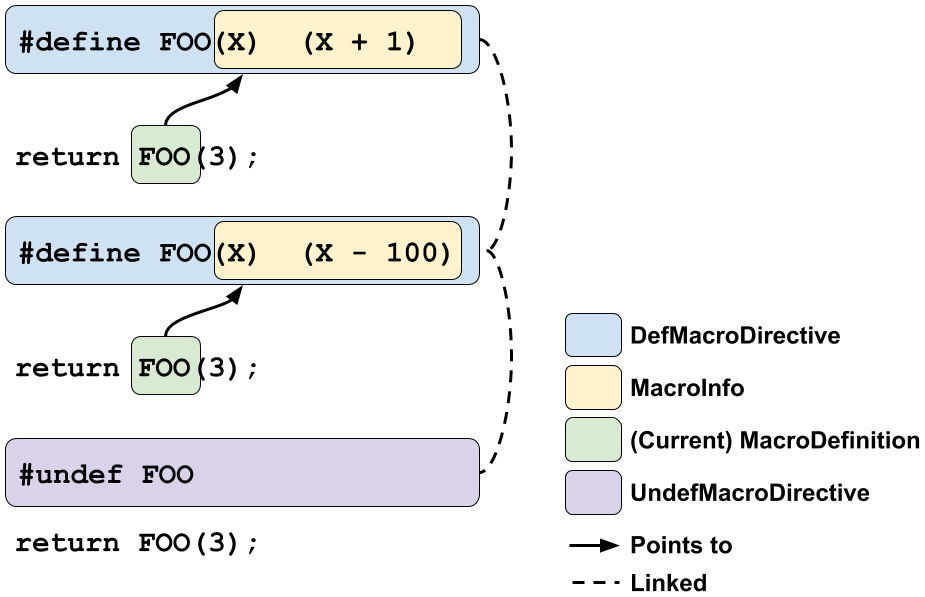
\includegraphics[width=0.9\textwidth]{content/2/chapter6/images/2.png}\\
图6.2 — C++中宏的类与前面的代码示例有何不同
\end{center}

要检索\texttt{MacroInfo}类和其\texttt{MacroDefinition}类,可以使用以下的预处理器API,如下所示:

\begin{lstlisting}[style=styleCXX]
void printMacroBody(IdentifierInfo *MacroII, Preprocessor &PP)
{
	MacroDefinition Def = PP.getMacroDefinition(MacroII);
	MacroInfo *Info = Def.getMacroInfo();
	…
}
\end{lstlisting}

前面的代码片段中显示的\texttt{IdentifierInfo}类型参数\texttt{MacroII}表示宏名。要进一步检查宏体,请运行以下代码:

\begin{lstlisting}[style=styleCXX]
void printMacroBody(IdentifierInfo *MacroII, Preprocessor &PP)
{
	…
	MacroInfo *Info = Def.getMacroInfo();
	for(Token Tok : Info->tokens()) {
		std::cout << Tok.getName() << "\n";
	}
}
\end{lstlisting}

通过本节,了解了\texttt{Preprocessor}的工作流程,以及两个重要组件:\texttt{Token}类和处理宏的子系统。了解这两种方法可以让您更好地了解Clang的预处理是如何工作的,并为下一节的\texttt{Preprocessor}插件和自定义回调开发做好准备。





























